\documentclass[runningheads]{llncs}
\protected\def\shortwordspace{\ifmmode\else~\fi}
%
\usepackage{graphicx}
\usepackage[utf8]{inputenc}
\usepackage[slovak]{babel}
\usepackage{multirow}
\newcommand\tab[1][0.5cm]{\hspace*{#1}}
\PassOptionsToPackage{hyphens}{url}\usepackage{hyperref}
%
\begin{document}

\authorrunning{Jozef Varga}
\titlerunning{Využitie genetického algoritmus na~výber atribútov}
%
\title{Využitie genetického algoritmu na~výber atribútov v oblasti behaviorálnej biometrie}
%
%
\author{Jozef Varga}
%
\institute{Fakulta informatiky a~informačných technológií \\
Slovenská technická univerzita v Bratislave\\
Ilkovičova 2, 842 16 Bratislava 4}
%
\maketitle              % typeset the header of the contribution
%
\begin{abstract}
    . Výber atribútov je v strojovom učení náročnou kombinatorickou úlohou. 
    Atribúty, ktoré neskôr vstupujú do rôznych modelov v strojovom učení, majú
    veľký vplyv na~následnú presnosť a~rýchlosť samotného modelu. Toto je jeden z~problémov,
    ktorý sa vyskytuje pri autorizovaní používateľa pomocou behaviorálnej biometrie. Práve pri
    zaznamenávaní dát o používateľovi získame veľké množstvo atribútov, ktoré znižujú rýchlosť výpočtu
    a~taktiež degradujú kvalitu klasifikácie. 
    
    \tab V tomto článku sme vytvorili genetický algoritmus, ktorý používame práve na~výber artibutov. Nami vytvorenú
    metódu porovnávame s bežnými metódami ako sú Variance Inflation Factor (VIF) a~výber atribútov pomocou korelácií (CORR). 
    Zvolené metódy boli porovnané pomocou rôznych klasifikátorov, ako sú napríklad K-Nearest Neighbors (KNN), SVM, Naive Bayes a~iné. 
    V práci sme využili verejný dataset~\cite{ref_dataset_anguita,ref_dataset}, ktorý obsahuje biometrické dáta o 
    používateľoch. Tieto dáta obsahujú informácie o tom, v akom stave sa nachádza používateľ, teda či leží, sedí, 
    kráča,  kráča hore schodami, kráča dole schodami alebo stojí.
    V tejto práci sa ukázalo, že použitie genetického algoritmu zlepšilo výsledky jednotlivých klasifikátorov a~
    má veľký potenciál, čo sa týka využitia, v tejto problematike.

\keywords{Behaviorálna biometria \and Genetický algoritmus \and Strojové učenie \and Výber funkcií / atribútov.}
\end{abstract}
%

%Úvod / Introduction - aká úloha sa ide riešiť, prečo je dobré ju riešiť
\section{Úvod}

V dnešnej dobe je využitie smartfónov na~vzostupe. 
Veľké množstvo ľudí tieto zariadenia využíva aj na~vyhľadávanie informácií, 
úpravu dokumentov a~rôzne ďalšie funkcionality, 
ktoré tieto zariadenia podporujú~\cite{ref_bomhold}. 
To, že sú smartfóny veľkou súčasťou technologického sveta potvrdzuje aj 
štatistika z~roku 2018, ktorá hovorí, že až 52,2\% 
zobrazení globálnych webových stránok prebiehalo pomocou mobilných zariadení. 
Zaujímavé je, že v tomto prípade ide o nárast až 51,5\% 
oproti štatistike z~roku 2009~\cite{ref_statista19}. Mobilné zariadenie
prináša veľmi veľa nových možností výskumu, ktoré sú orientované na~správanie človeka.
Dôvodom je hlavne veľké množstvo informácií, ktoré je možné vďaka senzorom v mobilnom 
zariadení zaznamenať. 

Tieto senzory zaznamenávajú takzvané biometrické črty.  
Biometria sa zakladá na~charakteristických črtách konkrétnej osoby. Tieto biometrické 
črty sa delia na~dva typy, a~to na~fyziologické a~behaviorálne 
(viď. Obr.~\ref{fig_rozdelenie_biometrie})~\cite{ref_teh}. Fyziologická biometria, 
ako napríklad odtlačok prsta, je veľmi často využívanou overovacou technikou, 
keďže je jedinečná a~stála. Táto biometria má však aj svoje nevýhody. 
DNA, čo je typickým príkladom tejto biometrie, je dosť invazívne na~to, 
aby sa využívalo napríklad na~smartfónoch, keďže jej využitie by 
vyžadovalo určitú podmienenú činnosť používateľa, napríklad odber krvi. 
Naopak behaviorálna biometria má výhodu v možnosti práce na~pozadí bez akejkoľvek 
určitej požadovanej činnosti užívateľa. Keďže sa jedná o charakteristiky, 
ako napríklad rýchlosť písania, nakláňanie smartfónu alebo chôdza, 
používateľove správanie môže byť overené počas bežných činností ~\cite{ref_teh}.
Výhodou behaviorálnych čŕt je teda fakt, 
že ak už zariadenie disponuje potrebným hardvérom, 
v prípade mobilných zariadení napríklad senzormi, 
je možné vykonávať rôzne operácie, ako napríklad autentifikáciu používateľa alebo 
identifikovanie stavu, v akom sa používateľ nachádza, bez toho, aby o 
tom samotný používateľ vedel. Naopak nevýhodou tejto biometrie je, 
že behaviorálne charakteristiky používateľa sa časom menia, 
a teda je potrebné častejšie vytvorenie profilu používateľa ~\cite{ref_seyd}. 

Jedným z~problémov, ktorý sa objavuje pri prácach s behaviorálnimi črtami, 
je množstvo atribútov, ktoré sa získavajú zo senzorov ~\cite{ref_nascimento}. 
Získané atribúty môžu obsahovať irelevantné/zavádzajúce informácie, ktoré
môžu mať za následok zníženie kvality klasifikácie modelu
~\cite{ref_babatunde,ref_lu,ref_nascimento,ref_smith,ref_zhao}. 

Práve výberom atribútov sa 
budeme v tejto práci bližšie zaoberať. Naša metóda na~výber atribútov spočíva vo využití 
genetického algoritmu, ktorý bude aplikovaný na~výber čŕt v datasete, ktorý sa venuje skúmaniu
stavu používateľa (leží, chodí, sedí) na~základe biometrických črt získaných z~
mobilného zariadenia ~\cite{ref_dataset_anguita,ref_dataset}.


\begin{figure}
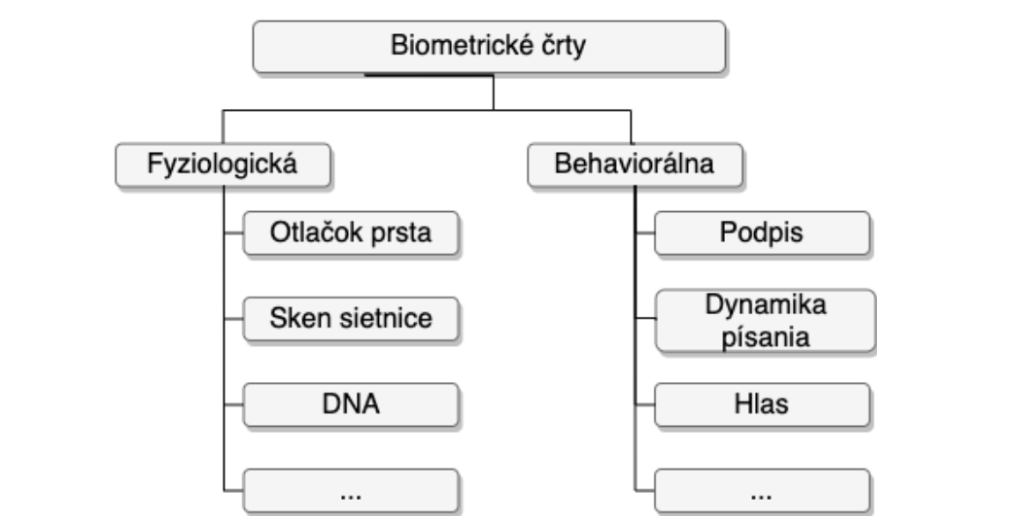
\includegraphics[width=\textwidth]{image/rozdelenie_biometrie.png}
\caption{Typy biometrických čŕt~\cite{ref_teh}.} \label{fig_rozdelenie_biometrie}
\end{figure}

%Podobné práce / Related Work - ako riešili vašu alebo podobnú úlohu vexistujúcich prácach - nezabudnite v texte uvádzať citácie na~práce.
\section{Podobné práce}

Výber atribútov je veľmi podstatnou časťou pri strojovom učení. Veľmi veľa prác sa 
zaoberá rôznymi metódami, ktoré by boli nápomocné pri spracovávaní rôznych datasetov.
V práci ~\cite{ref_nascimento} experimentovali nad dvoma databázami, pričom 
prvá databáza mala 43 atribútov a~231 záznamov. Druhá databáza obsahovala 60 atribútov 
a 7555 záznamov. Dáta si rozdelili na~testovaciu a~trénovaciu množinu v pomere 66:33. 
Na trénovanie modelu bolo určených 66\% dát a~33\% dát sa použilo na~jeho testovanie. 
V práci využívajú na~klasifikáciu metódu k~najbližších susedov (angl. K-Nearest Neighbors, skr. KNN), metódu podporných vektorov (angl. support vector machines, skr. SVM) a~Naivný Bayesovský klasifikátor (angl. Naive Bayes)  
(pozri. Tab.~\ref{tab_vyber_funkci}). Na konci experimentu autori zhodnotili, 
že využitie genetického algoritmu na~výber atribútov pri rôznych klasifikátoroch malo veľmi priaznivé
účinky práve na~SVM, a~to v zlepšení až o 14,55\% v prvom datasete a~11,77\% v druhom datasete.
Keďže zlepšenie bolo výrazné pri každom zo spomenutých klasifikátorov, autori v práci usúdili, že
využitie genetických algoritmov v tejto problematike zvyšuje presnosť klasifikátora.

\begin{table}[]
\centering
\caption{Presnosť (angl. accuracy, skr. ACC) modelov výberu funkcií v percentách ~\cite{ref_nascimento}.}\label{tab_vyber_funkci}
\begin{tabular}{|c|c|c|c|}
\hline
                     & \multicolumn{3}{c|}{\textbf{Bez výberu funkcií}}                     \\ \hline
\textbf{Databáza}    & \textbf{KNN}          & \textbf{SVM}          & \textbf{Naive Bayes} \\ \hline
Da Silva et al. 2016 & 72,73 ± 2,74           & 73,55 ± 2,63           & 55,54 ± 3,54           \\ \hline
Giot et al. 2009     & 86,72 ± 0,58           & 78,28 ± 0,67           & 69,33 ± 0,67          \\ \hline
\textbf{Databáza}    & \multicolumn{3}{c|}{\textbf{Využitie genetického algoritmu na~výber funkcií}} \\ \hline
Da Silva et al. 2016 & 87,85 ± 0,84            & 88,10 ± 0,90           & 81,64 ± 0,97          \\ \hline
Giot et al. 2009     & 88,86 ± 0,23           & 90,05 ± 0,41            & 77,44 ± 0,27          \\ \hline
\end{tabular}
\end{table}


V práci \cite{ref_babatunde} autori využili na~výber atribútov tri rôzne algoritmy, a~to 
genetický algoritmus, Waikato pre analýzu znalostí - výber prvkov založený na~korelácii (angl. Waikato Environment for Knowledge Analysis - Correlation-based Feature Selection, skr. WEKA-CFS) a~Waikato pre analýzu znalostí - výber prvkov založený na~hodnotení (angl. Waikato Environment for Knowledge Analysis - ranker, skr. WEKA-ranker). Na vyhodnotenie taktiež použili viacero klasifikátorov
a to viac vrstvový perceptron (angl. Multi-Layer Perceptron, skr. MLP ), náhodný les (angl. Random Forest, skr. RF), J48, Naive Bayes a~regresiu. Najlepšie výsledky 
boli získané pomocou MLP. Ako najlepšia funkcia na~výber atribútov sa ukázal práve genetický algoritmus,
ktorý má výhodu v širokej možnosti nastavovania.

Práca \cite{ref_zhao} využila genetický algoritmus na~optimalizáciu nielen výberu atribútov, 
ale aj výberu parametrov pre SVM klasifikátor. Využitie tohto algoritmu, nielen zlepšilo výsledky klasifikácie, 
ale oproti  grid searchu aj zrýchlilo výpočet o 2,62 sekundy.
Presnosť klasifikácie sa zvýšila až o 3,57\%. Najnižšie 
získané hodnoty 83,14 ± 7,19 boli s využitím výberu atribútov založenom na~genetickom algoritme.

Práca \cite{ref_smith} sa zaoberala predovšetkým klasifikátorom C4.5.
Autori v nej skúmali ako vplýva genetický algoritmus, ktorého fitness funkcia pozostáva zo stromu, 
na výber atribútov aj u iných algoritmov. Vo fitness funkcii teda neskúšali využívať len
klasifikátor, s ktorým neskôr prebieha klasifikácia. Zistili, že takáto fitness funkcia,
taktiež zlepšuje aj iné modely. Ich výsledky ukázali, že ak rovnakú funkciu použili na~
Naive Bayes, tak jeho klasifikácia sa zlepšila o 4,92 \%.

Nami vytvorený genetický algoritmus chceme porovnať s existujúcimi algoritmami na~výber 
atribútov, a~to faktor inflácie (angl. Variance Inflation Factor, skr. VIF) a~výber atribútov na~základe korelácií (skr. CORR).  
Na fitness funkciu chceme využiť len jeden algoritmus, a~to K-Nearest Neighbors (KNN), ako bude spomenuté v nasledujúcej kapitole.


%opis použitého algoritmu - aj s odôvodnením výberu algoritmu
\section{Využívané algoritmy na~výber atribútov}
V tejto práci sme sa rozhodli porovnať genetický algoritmus na~výber atribútov s
algoritmami Variance Inflation Factor (VIF) a~výberom na~základe korelácií (CORR). Tieto 
algoritmy sa radia medzi základné algoritmy na~výber atribútov \cite{ref_xu}.
\subsection{Variance Inflation Factor}
Tento algoritmus odstraňuje atribúty, ktoré majú veľmi silnú kolinearitu.
VIF odhaduje do akej miery je rozptyl koeficientu zväčšený kvôli lineárnej závislosti
s iným prediktorom. Výpočet VIF pre každý stĺpec (1) sa dá získať vykonaním lineárnej 
regresie tohto stĺpca so všetkými ostatnými stĺpcami \cite{ref_xu}.

\begin{equation}
VIF_{i}=\frac{1}{1-R_{i}^{2}}
\end{equation}    
V uvedenom vzorci \begin{math}R_i^2\end{math} predstavuje koeficient regresie medzi i-tou premennou a~
všetkými ostatnými premennými. VIF sa pri výbere atribútov porovnáva a~odstraňujú sa hraničné hodnoty \cite{ref_xu}.

\subsection{Výber atribútov na~základe korelácií}
Atribúty sú vyberané na~základe korelačného koeficientu. Koeficient korelácie je miera lineárnej intenzity 
korelácie. Najčastejšie je využívaný Pearsonov korelačný koeficient. Tento koeficient nadobúda hodnoty medzi
\begin{math}1\end{math} až \begin{math}-1\end{math}. \begin{math}1\end{math} vo výsledku predstavuje perfektnú pozitívnu 
koreláciu (podobnosť). Naopak \begin{math}-1\end{math} predstavuje 
perfektńu negatívnu koreláciu (podobnosť). \begin{math}0\end{math} označuje, že medzi prvkami nie je žiadna korelácia / podobnosť.
Cieľom tohto algoritmu je odstránenie takmer totožných stĺpcov.\cite{ref_xu}

\subsection{Genetický algoritmus}

Genetické algoritmy sú inšpirované evolúciou. Ich základ sa teda skladá z~generácií, ktoré sa vyvíjajú a~obsahujú 
určité množstvo chromozómov, ktoré sa spolu volajú populácia. Tieto chromozómy obsahujú kritické informácie 
potrebné na~vyriešenie problému. Tieto algoritmy sa využívajú najmä na~optimalizáciu rôznych
problémov. Ich uplatnenie je v praxi veľmi široké \cite{ref_babatunde,ref_whitley}. Nami vytvorený algoritmus začína 
inicializáciou populácie genetického algoritmu (Obr.~\ref{fig_ga_rozdelenie}).
\begin{figure}
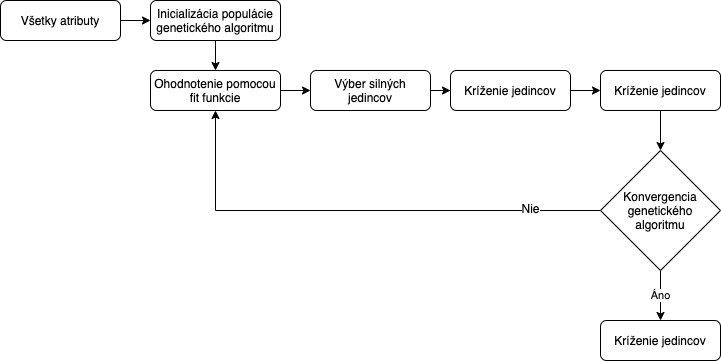
\includegraphics[width=\textwidth]{image/GA_alg.png}
\caption{Schéma genetického algoritmu na~výber atribútov.} \label{fig_ga_rozdelenie}
\end{figure}
    
\subsubsection{Inicializácia populácie genetického algoritmu.}

Pri inicializácií sa nastavia prvotné funkcie genetického algoritmu (Tab.~\ref{tab_nastavenie_gen_alg}). Nastavenie genetického algoritmu bolo na~základe testov a~opísaných prác ~\cite{ref_babatunde}.
V algoritme je chromozóm reprezentovaný \begin{math}n\end{math} génmi. Jeden gén prezentuje \begin{math}1\end{math} 
alebo \begin{math}0\end{math}, ktorá hovorí, či sa vo výslednom vektore atribútov nachádza alebo nie. 
Počet týchto génov \begin{math}n\end{math} je počtom atribútov, ktoré sú vo vstupnom vektore, a~teda 
koľko atribútov má daný dataset.

\begin{table}[]
\centering
\caption{Nastavenie genetického algoritmu.}\label{tab_nastavenie_gen_alg}
\begin{tabular}{|l|l|}
\hline
\textbf{Parametre GA}                    & \textbf{hodnota}  \\ \hline
Fitness funkcia založená na~modeli           & K-Nearest Neighbors~\cite{ref_babatunde} \\ \hline
Reprezentácia génu                       & Boolean  \\ \hline
Maximálny počet generácií                & 20       \\ \hline
Veľkosť populácie                        & 100      \\ \hline
Chromozómy vytvorené krížením            & 30       \\ \hline
Chromozómy vytvorené generovaním         & 30       \\ \hline
Najlepšie chromozómy z~minulej generácie & 20       \\ \hline
Percentuálna šanca mutácie a~kríženia    & 60\%     \\ \hline
\end{tabular}
\end{table}

\subsubsection{Ohodnotenie populácie pomocou fitness funkcie.}

Populácia, ktorá sa dostane do tohto kroku, musí byť ohodnotená pomocou fitness funkcie. 
Táto funkcia musí ohodnotiť jednotlivé chromozómy tak, aby bolo možné ich porovnať a~zistiť, ktorý
z týchto chromozómov je najúspešnejší. Táto fitness funkcia pozostáva z~priemeru ďesaťnásobnej krížovej validácie, ktorej jadro
je vytvorené z~KNN algoritmu. Najlepšie hodnotený chromozóm sa uloží ako aktuálny výsledok a~algoritmus pokračuje
na výber jedincov (chromozómov) do ďalšej generácie.

\subsubsection{Výber silných jedincov.}

Tento spôsob sa nazýva elitárstvo, teda koľko najlepších chromozómov z~predchádzajúcej generácie prejde
do novej generácie. Výhodou je najmä to, že silné jedince sa naďalej reprodukujú a~predávajú svoje vlastnosti
novovytvoreným chromozómom.

\subsubsection{Kríženie jedincov.}

Pri krížení sa spájajú vlastnosti dvoch jedincov do jedného (Obr.~\ref{fig_ga_krizenie}).
Do kríženia vstupujú dva chromozómy, ktoré majú zrkadlové postavenie v zoradenom liste podľa fitness funkcie. 
Jeden chromozóm je teda z~časti, kde je fitness funkcia najsilnejšia a~jeden z~časti, kde je fitness funkcia naopak slabšia. 
Tento spôsob by mal pomôcť algoritmu, aby nezastal na~lokálnom maxime. Následne sa prechádza po génoch 
jednotlivých chromozómov a~podľa percentuálnej náhody sa vyberie jeden z~génov do budúceho jedinca.
Šanca, s akou sa jednotlivé gény volia, ako aj počet takto vytvorených jedincov sa v genetickom algoritme
nastavuje pomocou parametrov (Tab.~\ref{tab_nastavenie_gen_alg}). 

\begin{figure}
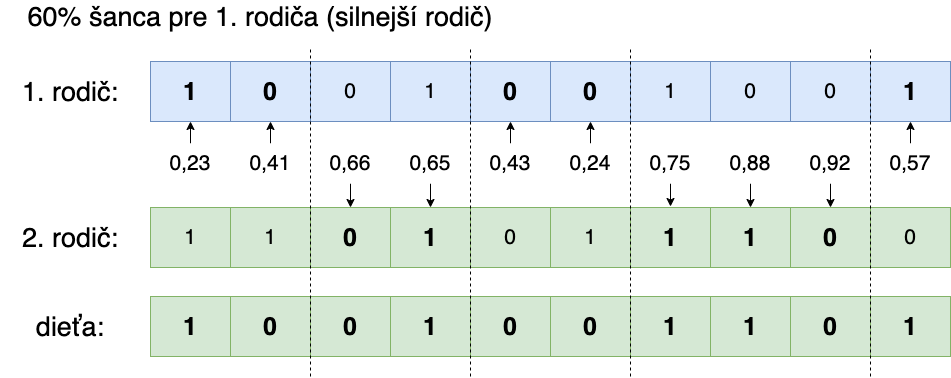
\includegraphics[width=\textwidth]{image/krizenie.png}
\caption{Kríženie chromozómov.} \label{fig_ga_krizenie}
\end{figure}

Zvyšné chromozómy sa náhodne vygenerujú ako pri inicializácií, aby počet chromozómov v každej generácií bol rovnaký. 
Ako posledné prejde algoritmus k~mutácii. Tá prejde všetky chromozómy v zadanej populácií a~následne aj jednotlivé gény.
Nad každým génom sa vygeneruje náhodné číslo, na~základe ktorého sa s 60\% šancou gén zmení na~opačný (Obr.~\ref{fig_ga_mutovanie}). 

\begin{figure}
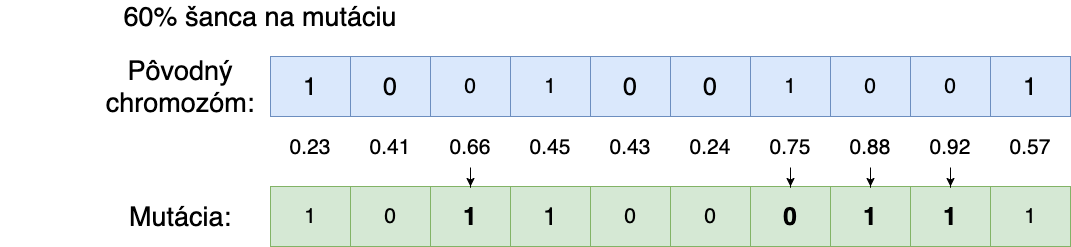
\includegraphics[width=\textwidth]{image/mutacia.png}
\caption{Mutácia chromozómov.} \label{fig_ga_mutovanie}
\end{figure}




%opis vykonaných experimentov - opis použitého datasetu, opis cieľu a~postupuexperimentu, opis nastavení algoritmu (odôvodnenie prečo zvolené nastavenia), opis metrík, ktorými experiment vyhodnocujete... ak sa porovnávate s existujúcimi riešeniami, nezabudnite ich citovať, prípadne aj stručne opísať
\section{Experimenty}

Konfigurácia genetického algoritmu zobrazená v tabuľke~\ref{tab_nastavenie_gen_alg} bola zvolená na~
základe pilotných testov nad rôznymi dátami. V experimente využijeme dataset, ktorý obsahuje behaviorálne 
záznamy z~mobilného zariadenia~\cite{ref_dataset_anguita,ref_dataset}. Tento dataset slúži na~klasifikovanie
stavu používateľa, a~teda či používateľ leží, sedí, kráča, kráča hore schodami, kráča dole schodami alebo stojí.
Dataset obsahuje informácie o 30 dobrovoľníkoch vo veku 19 až 48 rokov. Každý používateľ vykonal spomenutých
6 aktivít, pri ktorých mal na~páse pripevnený smartfón Samsung Galaxy S II. Dataset obsahuje informácie z~
gyroskopu a~akcelerometra. Z~nich sa zaznamenávalo 3-osové lineárne zrýchlenie a~3-osové uhlové rýchlosti 
pri~konštantných 50 Hz. V datasete sa nachádza 3609 záznamov. Každý záznam v datasete obsahuje 561 atribútov, ktoré obsahujú:

\begin{itemize}
\item trojosové zrýchlenie z~akcelerometra a~odhadované zrýchlenie tela,
\item trojosovú uhlovú rýchlosť z~gyroskopu,
\item označenie činnosti,
\item označenie konkrétneho subjektu.
\end{itemize}

Nad týmto datasetom sa snažíme overiť a~porovnať silu genetického algoritmu oproti štandardným metódam. Porovnávame 
jeho získané accurancy skóre so skóre, ktoré získa algoritmus VIF alebo analýza na~základe korelácií. V experimente boli využité modely
adaptívne zvýšenie
(angl. Adaptive Boosting, skr. AdaBoost), Rozhodovací strom (angl. Decision Tree), extrémne náhodné lesy (angl. Extra Trees), Naive Bayes, K-Nearest Neighbors, Lineárna diskriminačná analýza (angl. Linear Discriminant Analysis, skr. LDA), 
Logistická regresia (angl. Logistic Regression), neurónové siete (angl. Artificial neural networks, skr. ANN), Random Forest, SVM Sigmoid, SVM RBF a Kvalitatívna analýza údajov (angl. Qualitative Data Analysis, skr. QDA).

\subsection{Algoritmus na vyhodnocovanie.}

Na vyhodnocovanie sme použili algoritmus skúmajúci presnosť (angl. Accuracy, skr. ACC).Presnosť je jedným z najbežnejšie používaných algoritmov na vyhodnocovanie klasifikácie a je definovaná ako pomer medzi správne klasifikovanými vzorkami k celkovému počtu vzoriek. 
Vo vzorci (2) P a N označuje počet pozitívnych a negatívnych vzoriek. ~\cite{ref_sokolova}

\begin{equation}
Acc = \frac{TP+TN}{TP+TN+FP+FN}
\end{equation}  

\subsection{Implementácia.}

Hore spomenuté algoritmy strojového učenia, boli využité vďaka knižniciam sklearn a statsmodels. Genetický algoritmus je vytvorený podľa návrhu, ktorý je spomenutý vyššie. VIF a CORR je implementovaný čiastočne nami a čiastočne pomocou uvedených knižníc. Pri algoritme CORR využívame z knižníc funkciu corr, ktorá nám vracia hodnotu korelácie a pri VIF sa využíva funkcia variance\_inflation\_factor, ktorá nám vráti výsledok variancie pre jednotlivý stĺpec. Ostatné časti na odstraňovanie atribútov sú vytvorené nami.

%Vyhodnotenie / Evaluation - prehľadné výsledky experimentov (formou textového opisu, grafov, tabuliek, ...)
\section{Vyhodnotenie}

Výsledky experimentu sú zobrazené v tabuľke ~\ref{tab_nastavenie_vyhodnotenie_experimentu} 
a tabuľke ~\ref{tab_pocet_vyber_atributov} . Využitie genetického algoritmu
nám v tomto experimente ukázalo, že časovo najnáročnejší na~predspracovanie bol algoritmus 
VIF. Oproti GA bol tento algoritmus až 13-krát pomalší (tabuľka~\ref{tab_cas_vyber_atributov}). Ak sa predpokladá zlepšenie GA zvýšením počtu generácií, vieme povedať, že výsledky GA je ešte možné zlepšiť 
zvýšením jeho časového zaťaženia. 


\begin{table}[]
    \centering
    \caption{Výsledky genetického algoritmu. Jadro funkcie bolo KNN}\label{tab_nastavenie_vyhodnotenie_experimentu}
    \begin{tabular}{|l|c|c|c|c|c|c|}   
    \hline
    \textbf{Model}               & \multicolumn{3}{c|}{\textbf{ACC}}                       & \textbf{ Najlepší  } \\ 
                                 & \textbf{GA} & \textbf{VIF} & \textbf{CORR}& \textbf{výsledok}  \\ \hline
    AdaBoost                     & 0,54        & 0,55         & 0,54       & VIF   \\ \hline
    Decision Tree                & 0,84        & 0,85         & 0,84       & VIF     \\ \hline
    Extra Trees                  & 0,77        & 0,70         & 0,68       & GA       \\ \hline
    Naive Bayes                  & 0,79        & 0,87         & 0,81       & VIF        \\ \hline
    Nearest Neighbors            & 0,92        & 0,14         & 0,14       & GA            \\ \hline
    Linear Discriminant Analysis & 0,95        & 0,95         & 0,94       & GA, VIF              \\ \hline
    Logistic Regression          & 0,95        & 0,96         & 0,95       & VIF         \\ \hline
    Neural Net                   & 0,94        & 0,71         & 0,69       & GA           \\ \hline
    Random Forest                & 0,73        & 0,70         & 0,70       & GA              \\ \hline
    SVM Sigmoid                  & 0,19        & 0,19         & 0,19       & Všetky         \\ \hline
    SVM RBF                      & 0,21        & 0,19         & 0,19       & GA           \\ \hline
    QDA                          & 0,87        & 0,91         & 0,87       & VIF           \\ \hline
    \end{tabular}
\end{table}


Čo sa týka počtu atribútov, každý z~použitých algoritmov znížil počet atribútov o viac ako polovicu, čím sa znížil čas následného 
trénovania. Najviac atribútov vyfiltroval VIF, a~to až o 70 atribútov viac ako GA. 
Zaujímavosťou je práve GA, ktorý potvrdzuje, že výberom správneho algoritmu 
do~fitness funkcie sa výrazne zlepší výsledná klasifikácia modelu, ktorý je použitý
ako základ tejto funkcie. Získané výsledky taktiež ukazujú, že nie je potrebné, aby sa 
zhodovalo jadro fitness funkcie s modelom, ktorý je klasifikátorom. Toto je vidieť 
hlavne pri modeloch ANN a~QDA, kde aj pri použití fitness funkcie s jadrom 
K-Nearest Neighbors sa zvýšila klasifikácia týchto modelov o viac ako 15\% oproti 
klasifikácii nad neupravenými atribútmi. Najväčšie zlepšenie je vidieť na~algoritme 
K-Nearest Neighbors, kde sa klasifikácia zlepšila o 78\%. Dôvodom je práve využitie tohoto algoritmu vo fitness funkcii.
Výsledky taktiež ukazujú, že ak bol VIF oproti GA lepší, rozdiel bol najviac 1\% okrem QDA, 
kde bol rozdiel 4\% a~Naive Bayes s rozdielom 8\%. Tieto rozdiely môžu byť zanedbateľné v prípade, ak
je potrebné znížiť časové zaťaženie na~predspracovanie, keďže VIF je 13krát pomalší.

\begin{table}[]
    \centering
    \caption{Počet vybratých atribútov. Jadro fitness funkcie bolo KNN}\label{tab_pocet_vyber_atributov}
    \begin{tabular}{|l|c|c|c|c|}
    \hline
    \textbf{Algoritmus}                  & GA        & VIF         & CORR          & Bez funkcie výberu \\ \hline
    \textbf{Počet atribútov}            & 260        & 190         & 255          & 562 \\ \hline
    \end{tabular}
\end{table}

\begin{table}[]
    \centering
    \caption{Čas trvania jednotlivých algoritmov na výber atribútov. Jadro fitness funkcie bolo KNN}\label{tab_cas_vyber_atributov}
    \begin{tabular}{|l|c|c|c|c|}
    \hline
    \textbf{Algoritmus}                  & GA        & VIF         & CORR          & Bez funkcie výberu \\ \hline
    \textbf{Počet atribútov}            & 5364,672s        & 71266,493s         & 2,403s          & 0,009s \\ \hline
    \end{tabular}
\end{table}

%Záver / Conclusion
\section{Záver}


Ako už bolo uvedené vo vyhodnotení, experiment sa uskutočnil nad existujúcim datasetom, 
ktorý obsahoval behaviorálne dáta o stavoch používateľov~\cite{ref_dataset_anguita,ref_dataset}.
Dataset bol vyhodnocovaný pomocou 11 modelov, a~desaťnásobnej krížovej validácie.
Podľa výsledkov uvedených v tabuľke~\ref{tab_nastavenie_vyhodnotenie_experimentu} 
a tabuľke~\ref{tab_pocet_vyber_atributov} je možné pozorovať, že využitie rovnakého klasifikátora
ako je použitý vo fitness funkci, je veľmi účinné a~zvyšuje presnosť klasifikácie. Využitie aj iného klasifikátora má za následok zlepšenie klasifikácie, avšak toto zlepšenie nie je až tak výrazné. Uspešné zníženie počtu atributov má za následok zrýchlenie následnej klasifikácie. Ďalším zistením je, že klasifikáciu je možné zlepšiť 
využitím genetického algoritmu oproti klasifikácii neupravených dát. 

Proces výberu atribútov je jedným z~najdôležitejších krokov v predspracovaní údajov. Datasety 
obsahujúce behaviorálne dáta obsahujú veľmi veľa atribútov, čo môže vyžadovať vysokú výpočtovú silu. V našom
experimente je taktiež vidieť, že GA znížilo počet atribútov o viac ako polovicu s tým, že presnosť klasifikátora sa zvýšila.
Práve preto môže výber atribútov, ktoré sú podstatné pre~klasifikáciu, zvýšiť presnosť klasifikácie
ako je ukázané vyššie. Použitie genetických algoritmov sa zdá byť lepšie aj oproti VIF vďaka nižšej časovej záťaži.
Najlepší klasifikátor pre náš dataset bol Logistic Regression a~LDA s 95\%. Medzi najlepšie tiež patria
ANN s 94\% a~KNN s 92\%.

Ďalšie pokračovanie tejto práce by bolo zamerané na~zmeny fitness funkcie, pričom cieľom by bolo sledovať presnosť výsledkov ostatných modelov.

%Použitá literatúra / References - používajte LNCS štýl odkazovania sa nazdroje, pokyny nájdete aj v šablóne
\begin{thebibliography}{8}

\bibitem{ref_dataset_anguita}
Anguita, D. et al.: A public domain dataset for human activity recognition using smartphones. ESANN 2013 proceedings, 21st Eur. Symp. Artif. Neural Networks, Comput. Intell. Mach. Learn. April, 437–442 (2013).

\bibitem{ref_babatunde}
Babatunde, O. et al.: A Genetic Algorithm-Based Feature Selection. Int. J. Electron. Commun. Comput. Eng. 5, 4, 899–905 (2014).

\bibitem{ref_bomhold}
Bomhold, C.R.: Educational use of smart phone technology: A survey of mobile phone application use by undergraduate university students. Program. 47, 4, 424–436 (2013). \doi{10.1108/PROG-01-2013-0003}.

\bibitem{ref_lu}
Lu, H. et al.: A hybrid feature selection algorithm for gene expression data classification. Neurocomputing. 256, 2017, 56–62 (2017). \doi{10.1016/j.neucom.2016.07.080}.

\bibitem{ref_nascimento}
Nascimento, L.D.O. et al.: An investigation of genetic algorithm-based feature selection techniques applied to keystroke dynamics biometrics An investigation of genetic algorithm-based feature selection techniques applied to keystroke dynamics biometrics. SBSeg, 2–5 (2019).

\bibitem{ref_smith}
Smith, M.G., Bull, L.: Genetic programming with a genetic algorithm for feature construction and selection. Genet. Program. Evolvable Mach. 6, 3, 265–281 (2005). \doi{10.1007/s10710-005-2988-7}.


\bibitem{ref_sokolova}
sokolova, M., Japkowicz, N., Szpakowicz, S.: Beyond accuracy, F-score and ROC: a family of discriminant measures for performance evaluation. In: Australasian joint conference on artificial intelligence. Springer, Berlin, Heidelberg, 2006. p. 1015-1021.


\bibitem{ref_seyd}
Syed, Z. et al.: Touch gesture-based authentication on mobile devices: The effects of user posture, device size, configuration, and inter-session variability. J. Syst. Softw. 149, 158–173 (2019). \doi{10.1016/j.jss.2018.11.017}.

\bibitem{ref_statista19}
statista.com, 2018. Percentage of all global web pages served to mobile phones from 2009 to 2018. \url{https://www.statista.com/statistics/241462/global-mobile-phone-website-traffic-share/}. Posledny prístup 10 Marca 2020

\bibitem{ref_teh}
Teh, P.S. et al.: A survey of keystroke dynamics biometrics. Sci. World J. 2013, (2013). \doi{10.1155/2013/408280}.

\bibitem{ref_dataset}
UC Irvine Machine Learning Repository, \url{https://archive.ics.uci.edu/ml/datasets/human+activity+recognition+using+smartphones}. Posledny prístup 10 Marca 2020

\bibitem{ref_whitley}
Whitley, D.: A genetic algorithm tutorial. Stat. Comput. 4, 2, 65–85 (1994). \doi{10.1007/BF00175354}.

\bibitem{ref_xu}
Xu, J. et al.: Methods for performing dimensionality reduction in hyperspectral image classification. (2018). \doi{10.1177/0967033518756175}.

\bibitem{ref_zhao}
Zhao, M. et al.: Feature selection and parameter optimization for support vector machines: A new approach based on genetic algorithm with feature chromosomes. Expert Syst. Appl. 38, 5, 5197–5204 (2011). \doi{10.1016/j.eswa.2010.10.041}.

\end{thebibliography}

\end{document}
